\documentclass{article}

\usepackage[utf8]{inputenc}
\usepackage{amsthm}
\usepackage{amssymb}
\usepackage{mathtools}
\usepackage{graphicx}
\usepackage{mdframed}
\usepackage{float}
\usepackage[top=0.75in, bottom=0.75in, left=0.75in, right=0.75in]{geometry}
\usepackage{gauss}

\usepackage{array}
\allowdisplaybreaks

\makeatletter
\newcounter{elimination@steps}
\newcolumntype{R}[1]{>{\raggedleft\arraybackslash$}p{#1}<{$}}
\def\elimination@num@rights{}
\def\elimination@num@variables{}
\def\elimination@col@width{}
\newenvironment{elimination}[4][0]
{
    \setcounter{elimination@steps}{0}
    \def\elimination@num@rights{#1}
    \def\elimination@num@variables{#2}
    \def\elimination@col@width{#3}
    \renewcommand{\arraystretch}{#4}
    \start@align\@ne\st@rredtrue\m@ne
}
{
    \endalign
    \ignorespacesafterend
}
\newcommand{\step}[2]
{
    \ifnum\value{elimination@steps}>0\sim\quad\fi
    \left[
        \ifnum\elimination@num@rights>0
            \begin{array}
            {@{}*{\elimination@num@variables}{R{\elimination@col@width}}
            |@{}*{\elimination@num@rights}{R{\elimination@col@width}}}
        \else
            \begin{array}
            {@{}*{\elimination@num@variables}{R{\elimination@col@width}}}
        \fi
            #1
        \end{array}
    \right]
    & 
    \begin{array}{l}
        #2
    \end{array}
    \addtocounter{elimination@steps}{1}
}
\makeatother

\DeclarePairedDelimiter{\abs}{\lvert}{\rvert}
\DeclarePairedDelimiter{\norm}{\lvert \lvert}{\rvert \rvert}

\newtheoremstyle{break}% name
  {}%         Space above, empty = `usual value'
  {}%         Space below
  {\itshape}% Body font
  {}%         Indent amount (empty = no indent, \parindent = para indent)
  {\bfseries}% Thm head font
  {.}%        Punctuation after thm head
  {\newline}% Space after thm head: \newline = linebreak
  {}%         Thm head spec

\newtheorem{Def}{Definition}[section]

\theoremstyle{break}

\newtheorem{innerEx}{Exempel}[section]
\newtheorem{sats}{Sats}[section]
\newtheorem{Rem}{Anmärkning}[]

\newenvironment{Ex}
{\begin{mdframed} \begin{innerEx} \vspace{3pt}}
{\vspace{3pt} \end{innerEx} \end{mdframed}}  

\newenvironment{bevis}
{\begin{mdframed} \begin{proof} \vspace{3pt}}
{\vspace{3pt} \end{proof} \end{mdframed}}


\title{
	 Linjär Algebra\\
	 Föreläsning 17 
    \author{Erik Sjöström}
}
\begin{document}
\maketitle

\section{Egenvärden (forts)} % (fold)
\label{sec:egenv_rden}
Bestäm en vektor $\vec{v} \neq \emptyset$ och ett tal $\lambda$ så att:
\[
\mathbf{A} \cdot \vec{v} = \lambda \cdot \vec{v}
\]
Om $\mathbf{A}^{T} \neq \mathbf{A}$ (osymmetrisk) och egenvärdena är multipla, så kan egenvektorerna tillhörande samma egenvärden sammanfalla.
\begin{Ex}
	För
	\[
	A ) \begin{bmatrix} 2&-1\\1&0 \end{bmatrix}
	\]
	har vi:
	\[
	0 = \mathbf{det}(\mathbf{A} - \lambda \cdot \mathbf{I}) = 
	\mathbf{det}
	\begin{pmatrix}
		\begin{bmatrix} 2&-1\\1&0 \end{bmatrix}
		- \lambda \begin{bmatrix} 1&0\\0&1 \end{bmatrix}
	\end{pmatrix}
	= \mathbf{det}
	\begin{pmatrix}
		\begin{bmatrix} 2- \lambda & -1\\1& - \lambda \end{bmatrix}
	\end{pmatrix}
	= (2 - \lambda)\cdot(-\lambda)-n \cdot (-1) = (\lambda - 1)^2
	\]
	\[
	\begin{cases}
		\lambda_1 = 1\\
		\lambda_2 = 1
	\end{cases}
	\]
	Egenvektor:
	\begin{gather*}
		(A - \lambda \cdot \mathbf{I}) \cdot \vec{v} = (\mathbf{A} - \mathbf{I}) \cdot \vec{v} = \emptyset\\
		\Leftrightarrow
		\begin{pmatrix}
			\begin{bmatrix} 2 &-1\\1&0 \end{bmatrix} -
			\begin{bmatrix} 1&0\\0&1 \end{bmatrix}
		\end{pmatrix}
		\begin{bmatrix} v_1\\v_2 \end{bmatrix} = 
		\begin{bmatrix} 0\\0 \end{bmatrix}\\
		\Leftrightarrow \begin{bmatrix} 1&-1\\1&-1 \end{bmatrix}
		\begin{bmatrix} v_1\\v_2 \end{bmatrix} = 
		\begin{bmatrix} 0\\0 \end{bmatrix} \Rightarrow
		\begin{bmatrix} v_1\\v_2 \end{bmatrix} = 
		t \cdot \begin{bmatrix} 1\\1 \end{bmatrix} , t \neq 0
	\end{gather*}
	Vi får bara en egenvektor:
	\[
	\vec{v}_1 = \begin{bmatrix} 1\\1 \end{bmatrix} \cdot \frac{1}{\sqrt{2}}
	\]
\end{Ex}
Även om egenvärdena är multipla så behöver inte egenvektorerna sammanfalla.
\newpage
\begin{Ex}
	\[
	\mathbf{A} = \begin{bmatrix} 2&-1&1\\1&-2&1\\1&-3&2 \end{bmatrix}
	\]
	Egenvärdena:
	\begin{gather*}
		\mathbf{det}(\mathbf{A} - \lambda \cdot \mathbf{I}) = \mathbf{det}
		\begin{pmatrix}
			\begin{bmatrix}
				2 - \lambda& - 3 & 1\\
				1 & -2 -\lambda & 1\\
				1 & -3 & 2 - \lambda
			\end{bmatrix}
		\end{pmatrix} = ... = - \lambda(\lambda - 1)^2 = 0
	\end{gather*}
	Som har lösningen:
	\[
	\begin{cases}
		\lambda_1 = 0\\
		\lambda_2 = 1\\
		\lambda_3 = 1
	\end{cases}
	\]
	Egenvektorn som hör till $\lambda_1 0 0$ blir:
	\[
	\vec{v}_1 = \begin{bmatrix} 1\\1\\1 \end{bmatrix}
	\]
	Egenvektor för $\lambda_2, \lambda_3$:
	\begin{gather*}
		(\mathbf{A} - \lambda_2 \cdot \mathbf{I}) \cdot \vec{v} = 
		(\mathbf{A} - \mathbf{I}) \cdot \vec{v} = \emptyset\\
		\Leftrightarrow
		\begin{pmatrix}
			\begin{bmatrix}
				2 & -3 & 1\\
				1 & -2 & 1\\
				1 & -3 & 2	
			\end{bmatrix} - 
			\begin{bmatrix}
				1 & 0 & 0\\
				0 & 1 & 0\\
				0 & 0 & 1
			\end{bmatrix}
		\end{pmatrix}
		\begin{bmatrix} v_1\\v_2\\v_3 \end{bmatrix} = 
		\begin{bmatrix} 0\\0\\0 \end{bmatrix}\\
		\Leftrightarrow
		\begin{bmatrix}
			1 & -3 & 1\\
			1 & -3 & 1\\
			1 & -3 & 1
		\end{bmatrix}
		\begin{bmatrix} v_1\\v_2\\v_3 \end{bmatrix}
		= \begin{bmatrix} 0\\0\\0 \end{bmatrix}
	\end{gather*}
	Som har lösningarna
	\[
	s \cdot \begin{bmatrix} 3\\1\\0 \end{bmatrix} + t \cdot \begin{bmatrix} -1\\0\\1 \end{bmatrix}
	\]
	Vi har två linjärt oberoende egenvektorer (men säger att $\vec{v}_2, \vec{v}_3$ är en bas för egenrum, som hör samman med $\lambda_2 ,\lambda_3 = 1$)\\
	\begin{center}
		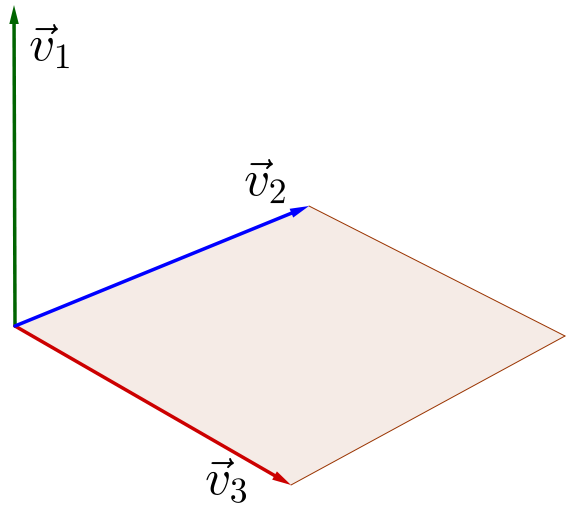
\includegraphics[scale=0.35]{bas.png}
	\end{center}
\end{Ex}
\paragraph{-} % (fold)
\label{par:_}
Mängden av egenvärden till en matris kallas för matrisens spektrum. Slutsatsen man kan dra om matrisens egenvärden kallas för spektralsatser.
% paragraph _ (end)	

\section{Spektralsatser} % (fold)
\label{sec:spektralsatser}
\begin{sats}
	En reell och symmetrisk matris \textbf{A} har alltid reella egenvärden.
\end{sats}
\begin{Ex}
	\[
	\mathbf{A} =
	\begin{bmatrix}
		6 & -2 & -1\\
		-2 & 6 & -1\\
		-1 & -1 & 5
	\end{bmatrix}
	\]
	\textbf{A} är symmetrisk. $(\mathbf{A}^T = \mathbf{A})$ och har reella egenvärden, $\lambda_1 = 8$, $\lambda_2 = 6$ och $\lambda_3 = 3$
\end{Ex}
\begin{sats}
	För en reell symmetrisk matris \textbf{A} gäller egenvärden tillhörande olika egenvärden är ortogonala (vinkelräta)
\end{sats}
\begin{Ex}
	\[
	\mathbf{A} =
	\begin{bmatrix}
		6 & -2 & -1\\
		-2 & 6 & -1\\
		-1 & -1 & 5
	\end{bmatrix}
	\]
	Har egenvektorerna:
	\begin{align*}
	& \vec{v}_1 = \overbrace{\begin{bmatrix} -1\\1\\0 \end{bmatrix}}^{\lambda_1 = 8}
	&& \vec{v}_2 = \overbrace{\begin{bmatrix} -1\\-1\\2 \end{bmatrix}}^{\lambda_2 = 6}
	&& \vec{v}_3 = \overbrace{\begin{bmatrix} 1\\1\\1 \end{bmatrix}}^{\lambda_3 = 3}
	\end{align*}
	Vi ser att:
	\begin{gather*}
		\vec{v}_1^T \cdot \vec{v}_2 =
		\begin{bmatrix} -1&1&0 \end{bmatrix} \cdot
		\begin{bmatrix} -1\\-1\\2 \end{bmatrix} = 
		(-1)^2 + (-1) + 0 = 0\\
		\vec{v}_1^T \cdot \vec{v}_3 =
		\begin{bmatrix} -1&1&0 \end{bmatrix} \cdot
		\begin{bmatrix} 1\\1\\1 \end{bmatrix} = ... = 0\\
		\vec{v}_2^T \cdot \vec{v}_3 = 
		\begin{bmatrix} -1&-1&2 \end{bmatrix} \cdot
		\begin{bmatrix} 1\\1\\1 \end{bmatrix} = ... = 0
	\end{gather*}
	De är alltså ortogonala mot varandra. 
\end{Ex}

\begin{sats}
	En reell symmetrisk matris \textbf{A} har alltid reella egenvärden och egenvektorerna $\vec{v}_i$ kan väljas ortogonal , dvs: parvis vinkelräta, ($\vec{v}_i^t \cdot \vec{v}_j = 0$ då $i = j$)
\end{sats}
Man kan formulera följande sammanfattning:
\begin{sats}
	Spektralsatsen för reella symmetriska matriser. Om \textbf{A} är en reell symmetrisk $(n \times n)$-matris, så gäller:
	\begin{itemize}
		\item \textbf{A} har \textit{n} reella egenvärden om man räknar multiplicitet.
		\item för varje egenvärde är egenrummets dimension samma som egenvärdets multiplicitet
		\item Egenrummen är parvis ortogonala och inom varje egenrum kan vi bilda en bas bestående av egenvektorer som är ortogonala mot varandra.
		\item \textbf{A} kan diagonaliseras $\mathbf{V}^T \mathbf{A} \mathbf{V} = \mathbf{D}$, med en en ortogonal matris \textbf{V}. Matrisen \textbf{V} har egenvektorer som kolonner och matrisen \textbf{D} har motsvarande egenvärden på diagonalen. 
	\end{itemize}
\end{sats}
% section spektralsatser (end)

\section{Diagonalisering} % (fold)
\label{sec:diagonalisering}

\begin{Ex}
	Titta på:
	\[
	\begin{bmatrix}
		6 & -2 & -1\\
		-2 & 6 & -1\\
		-1 & -1 & 5
	\end{bmatrix}
	\]
	Som har egenvärden $\lambda_1 = 8$, $\lambda_2 = 6$, och $\lambda_3 = 3$, och sammanhängande egenvektorer:
	\begin{align*}
	& \vec{v}_1 = \frac{1}{\sqrt{2}}\begin{bmatrix} -1\\1\\0 \end{bmatrix}
	&&\vec{v}_2 = \frac{1}{\sqrt{6}}\begin{bmatrix} -1\\-1\\2 \end{bmatrix}
	&&\vec{v}_3 = \frac{1}{\sqrt{3}}\begin{bmatrix} 1\\1\\1 \end{bmatrix}
	\end{align*}
	Med:
	\begin{align*}
	& \mathbf{V} = \begin{bmatrix} \vec{v}_1&\vec{v}_2&\vec{v}_3 \end{bmatrix}
	&&\mbox{ och }
	&& \mathbf{D} = 
	\overbrace{\begin{bmatrix}
		8 & 0 & 0\\
		0 & 6 & 0\\
		0 & 0 & 3
	\end{bmatrix}}^\text{egenvärden på diagonalen}
	\end{align*}
	Har vi:
	\[
	\mathbf{V}^T \cdot \mathbf{A} \cdot \mathbf{V} = D
	\]
	Alternativt:
	\begin{align*}
	& \mathbf{A} \cdot \vec{v}_1 = \lambda_1 \cdot \vec{v}_1
	&& \mathbf{A} \cdot \vec{v}_2 = \lambda_2 \cdot \vec{v}_2
	&& \mathbf{A} \cdot \vec{v}_3 = \lambda_3 \cdot \vec{v}_3
	\end{align*}
	\begin{gather*}
			\begin{bmatrix}
		\mathbf{A} \cdot \vec{v}_1 & 
		\mathbf{A} \cdot \vec{v}_2 & 
		\mathbf{A} \cdot \vec{v}_3
	\end{bmatrix}
	= 
	\begin{bmatrix}
		\lambda_1 \cdot \vec{v}_1&
		\lambda_2 \cdot \vec{v}_2&
		\lambda_3 \cdot \vec{v}_3
	\end{bmatrix}\\
	\Leftrightarrow
	\mathbf{A} \cdot 
	\overbrace{\begin{bmatrix}
		\vec{v}_1 & \vec{v}_2 & \vec{v}_3
	\end{bmatrix}}^{\mathbf{V}}
	= 
	\overbrace{\begin{bmatrix}
		\vec{v}_1 & \vec{v}_2 & \vec{v}_3
	\end{bmatrix}}^{\mathbf{V}}
	\cdot
	\overbrace{\begin{bmatrix}
		\lambda_1 & 0 & 0\\
		0 & \lambda_2 & 0\\
		0 & 0 & \lambda_3
	\end{bmatrix}}^{\mathbf{D}}
	\end{gather*}
	Kolumnerna i \textbf{V} har längden 1, de är parvis ortogonala.\\
	Dvs: ON-matris, dvs \textbf{V} är inverterbar och $\mathbf{V}^{-1} = \mathbf{V}^T$\\
	Multiplicera med $\mathbf{V}^T$ från vänster:
	\[
	\mathbf{V}^T \cdot \mathbf{A} \cdot \mathbf{V} = \overbrace{\mathbf{V}^T \cdot \mathbf{V}}^{\mathbf{I}} \cdot \mathbf{D} = \mathbf{D}
	\]
\end{Ex}
\begin{Def}
	En matris \textbf{A} är diagonaliserbar om det finns en inverterbar matris \textbf{P} och en diagonalmatris \textbf{D} sådan att:
	\[
	\mathbf{A} = \mathbf{P} \cdot \mathbf{D} \cdot \mathbf{P}^{-1}
	\]
\end{Def}
\begin{sats}
	En matris $\mathbf{A}_{n \times m}$ är diagonaliserbar om oom \textbf{A} har \textit{n} stycken linjärt oberoende egenvektorer.\\
	Då är:
	\begin{align*}
	&\mathbf{A} = \mathbf{V} \cdot \mathbf{D} \cdot \mathbf{V}^{-1}
	&&\mbox{eller}
	&&\mathbf{D} = \mathbf{V}^{-1} \cdot \mathbf{A} \cdot \mathbf{V}
	\end{align*}
	där \textbf{V}:s kolumner är egenvektorerna och diagonalen i \textbf{D} motsvarande egenvärden till \textbf{A} (i samma ordning).
\end{sats}
\paragraph{Obs:} % (fold)
\label{par:obs_}
Alla matriser kan inte diagonaliseras
% paragraph obs_ (end)
\begin{Ex}
	\[
	A = \begin{bmatrix} 2 & -1\\1&0 \end{bmatrix}
	\]
	hade $\lambda_1, \lambda_2 = 1$ och $\vec{v}_1 = \begin{bmatrix} 1\\1 \end{bmatrix}$ ej två stycken linjärt oberoende egenvektorer. Kan ej diagonaliseras. 
\end{Ex}
\begin{Ex}
	Låt \textbf{A} vara en inverterbar $(2 \times 2)$-matris med:
	\begin{align*}
	&\lambda_1 = 2 &&\vec{v}_1 = \begin{bmatrix} 1\\3 \end{bmatrix}\\
	&\lambda_2 = -1 &&\vec{v}_2 = \begin{bmatrix} 4\\1 \end{bmatrix}
	\end{align*}
	Bestäm egenvärden och egenvektorer till $\mathbf{A}^2$.
	\paragraph{Lösning:} % (fold)
	\label{par:l_sning_}
	\textbf{A} har två linjärt oberoende egenvektorer, alltså diagonaliserbar. Låt:
	\begin{align*}
	&\mathbf{V} = 
	\begin{bmatrix}
		\vec{v}_1 & \vec{v}_2
	\end{bmatrix}
	= 
	\begin{bmatrix}
		1 & 3\\
		3 & 1
	\end{bmatrix}
	&&\mbox{och}
	&&\mathbf{D} = 
	\begin{bmatrix}
		\lambda_1 & 0\\
		0 & \lambda_2
	\end{bmatrix}
	\end{align*}
	Vi har att:
	\begin{gather*}
		\mathbf{A} = \mathbf{V} \cdot \mathbf{D} \cdot \mathbf{V}^{-1}\\
		\mathbf{A}^2 = (\mathbf{V} \cdot \mathbf{D} \cdot \overbrace{\mathbf{V}^{-1}) \cdot (\mathbf{V}}^{\mathbf{I}} \cdot \mathbf{D} \cdot \mathbf{V}^{-1}) = \mathbf{V} \cdot \mathbf{D}^2 \cdot \mathbf{V}^{-1}\\
		\mathbf{D}^2 = \mathbf{D} \cdot \mathbf{D} = 
		\begin{bmatrix}
			2 & 0\\
			0 & -1
		\end{bmatrix} \cdot
		\begin{bmatrix}
			2 & 0\\
			0 & -1
		\end{bmatrix}
		=
		\begin{bmatrix}
			4 & 0\\
			0 & 1
		\end{bmatrix}
	\end{gather*}
	Dvs: $\mathbf{A}^2$ har egenvärden 4, 1, och egenvektorer:
	\begin{align*}
	&\vec{v}_1 = \begin{bmatrix} 1\\3 \end{bmatrix}
	&& \vec{v}_2 = \begin{bmatrix} 4\\1 \end{bmatrix}
	\end{align*}
	
	% paragraph l_sning_ (end)
\end{Ex}
% section diagonalisering (end)

% section egenv_rden (end)

\end{document}